\subsubsection{Clustering}
\label{subsec:03clustering}
Der finale Schritt der Bildverarbeitung besteht aus dem Clustering. Das Ziel ist die Bestimmung der Tiefe der Person aus der getrackten Bounding-Box mit m�glichst simplen und somit rechensparsamen Ans�tzen. Um �berhaupt Tiefeninformationen zu erhalten, wird ab diesem Schritt das Tiefenbild der Kinect-Kamera verwendet. Im ersten Schritt wird die Bounding-Box nach bestimmten Kriterien �berpr�ft, um den Voraussetzungen des an das Farbbild angepasste Tiefenbildes zu gen�gen. Die Voraussetzungen ergeben sich aus den unterschiedlichen Aufl�sungen von Farbbild und Tiefenbild und den schwarzen Bereichen an den R�ndern des Tiefenbildes, die durch dessen Verzerrung entstehen. Weiterhin werden invalide Tiefenbestimmungen aus dem Tiefenbild gefiltert, um ausschlie�lich brauchbare Werte in den n�chsten Verarbeitungsschritten zu ber�cksichtigen. \\
Aus den Tiefenpixel, die sich innerhalb der Bounding-Box befinden, wird nun der Mittelwert gebildet und anschlie�end eine Maske
\begin{align}
\text{Maske}(x,y)=\left\{\begin{matrix}
1 & \text{falls BBox}(x,y) &\leq \frac{1}{N_{x}+N_{y}} \sum_{x=0}^{N_{x}}\sum_{y=0}^{N_{y}}\text{BBox}(x,y)  \\ 
0 & \text{falls BBox}(x,y) &> \frac{1}{N_{x}+N_{y}} \sum_{x=0}^{N_{x}}\sum_{y=0}^{N_{y}}\text{BBox}(x,y)
\end{matrix}\right.
\end{align}
erstellt, die ausschlie�lich Pixel unterhalb des Mittelwertes ber�cksichtigt.
Maske$(x,y)$ und BBox$(x,y)$ beschreiben die Pixel der Maske bzw. Bounding-Box an der Stelle $(x,y)$ und $N_{x}$ bzw. $N_{y}$ die Anzahl der Pixel der jeweiligen Koordinatenrichtung. Der Gedanke hinter diesem Vorgehen ist, dass die Bounding-Box im Normalfall nur die Person und den Hintergrund enth�lt. Sollte dennoch zus�tzlich ein Hindernis in der Bounding-Box auftauchen, w�rde es nur einen kleinen Teil im Auschnitt ausmachen und somit die Maske kaum verf�lschen. In Abbildung \ref{fig:Maskierung} wird die Maskierung anhand eines Beispielbildes gezeigt.\\
Anschlie�end werden die Tiefeninformationen aus dem Tiefenbild, die sich innerhalb der Maske befinden, erneut gemittelt, um die gemittelte Tiefe der verfolgten Person zu erhalten. Zusammen mit dem Mittelpunkt des Detektionsfensters und der Projektionsmatrix der Kamera ergeben sich daraus die eindeutigen 3D-Koordinaten
\begin{equation}
\vec{P} =
\begin{pmatrix}
P_x\\P_y\\P_z
\end{pmatrix}
= p_z
\begin{pmatrix}
f_x & 0 & c_x\\
0 & f_y & c_y\\
0 & 0 & 1 
\end{pmatrix}^{-1}
\begin{pmatrix}
p_x\\p_y\\1
\end{pmatrix}
\end{equation}
der Person. Dabei entspricht $\vec{p}$ den Bildkoordinaten der Person, $\vec{f} = [f_x, f_y]^T$ der entsprechenden Brennweite und $\vec{c} = (c_x, c_y)^T$ dem Bildhauptpunkt.
\begin{figure}[h]
	\centering
	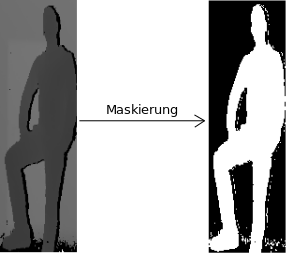
\includegraphics[width=0.4\textwidth]{pics/Maskierung.png}
	\caption{Die Maskierung der Bounding-Box des Tiefenbildes.}
	\label{fig:Maskierung}
\end{figure} \\